\section{Dataset Collection}

We use the Stack Exchange Data
Explorer\footnote{\texttt{https://data.stackexchange.com/stackoverflow/query/new}}
and construct a custom SQL query on the Stack Overflow data. The query could be
found under \texttt{source\_code/query.sql}.

The query satisfies the three requirements:

\begin{itemize}
    \item \texttt{\ldots select top 500} means that we are collecting at least
    500 threads.
    \item \texttt{\ldots Tags like \textquotesingle{}\%python\%\textquotesingle{}}
    means that we are collecting threads tagged \texttt{python}, discussing the
    Python programming language.
    \item \texttt{\ldots where AnswerCount >= 1} means we are collecting
    threads with at least 1 question and 1 answer.
\end{itemize}

The dataset contains 500 questions and 1254 answers, an average of 2.508 answers
per question. The distribution of answers is shown in Figure~\ref{ans-dist}.

\begin{figure}[h]
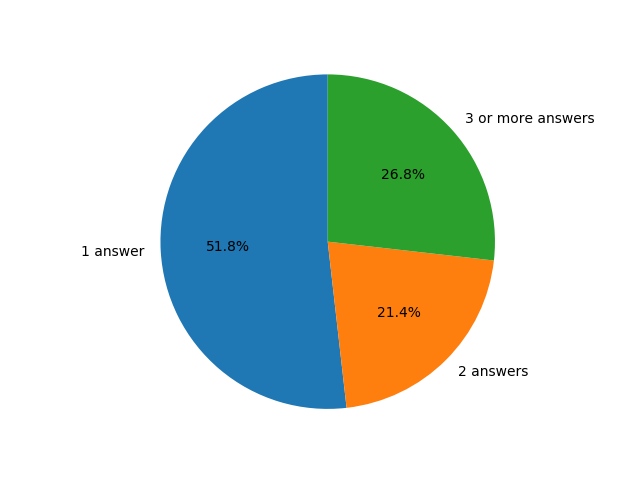
\includegraphics[width=0.9\linewidth]{no_ans_per_qn}
\caption{Distribution of answers}\label{ans-dist}
\end{figure}

\section{Dataset Analysis and Annotation}

\subsection{Stemming}

We used NLTK's~\cite{nltk} \texttt{PorterStemmer} to stem the dataset.
Prior to stemming, HTML tags and punctuations were removed, and stopwords
such as ``a'', ``of'' and ``the'' were also excluded from data, using the
stopwords corpus available in NLTK\@; this ensures that we are getting the
most meaningful words from the dataset. The top 20 words before and after
stemming are in Table~\ref{stem}.

\begin{table}
\caption{Top 20 words before and after stemming}\label{stem}
\begin{tabu}{X[1,l]X[4,l]|X[4,l]X[10,l]}
    \textbf{} & \textbf{Before stemming} &
    \textbf{After stemming} & \textbf{Original words} \\
    \midrule
    1 & I & I & I \\
    2 & Python & use &
    used, using, use, Use, useful, uses, Using, Usings \\
    3 & import & python &
    Python, Pythons, python, Pythonic, pythonic, pythons, pythonicity \\
    4 & use & import &
    import, imports, important, imported, Imported, importing, Import \\
    5 & 1 & 1 & 1 \\
    6 & def & def & def \\
    7 & You & return & 
    return, returns, returning, Returning, Returns, returned \\
    8 & return & file &
    files, file, File \\
    9 & using & tri &
    trying, tried, try, Try, tries, Trying, Tried \\
    10 & print & print &
    print, prints, printing, printed, Prints \\
    11 & like & you & You \\
    12 & code & like & 
    like, likes, likely, liked, Like \\
    13 & gtgtgt & code &
    code, coding, CODE, Code, Codes \\
    14 & class & list &
    list, Lists, lists, LIST, listing, List, listed \\
    15 & python & class &
    class, Class, classes, Classes \\
    16 & 2 & gtgtgt &
    gtgtgt, gtgtgts \\
    17 & list & function &
    function, functions, functionality, functional, Function \\
    18 & 3 & want &
    want, wanting, wants, wanted \\
    19 & want & valu &
    values, value, Values, Value \\
    20 & x & 2 & 2
\end{tabu} 
\end{table}

Using Porter Stemming algorithm, majority of the words retained their
semantic meaning after stemming. However, there were some irregularities
which caused the stemming to be incorrect.

Firstly in row 4, the word ``important'' was stemmed to the word ``import''.
This is an example of derivational suffix which not only changes the word class,
but also changes the semantic meaning of the word. Porter Stemming algorithm was
not able to capture the irregularity in this scenario. 

Looking at row 9, original words were variations of the word ``try''. After
stemming, all of them were stemmed to a single word, ``tri''. This word had a
meaning of ``three'' which was clearly different from ``try''. Porter Stemming
algorithm had mistakenly treated all variations of ``try'' as ``tri''.

Lastly, at row 19, variations of ``value'' were stemmed to the word ``valu''.
The word ``valu'' is not a proper English word. Porter Stemming algorithm had
generated a word that does not exist in the English dictionary.

\subsection{POS Tagging}

We picked 10 sentences at random and applied POS tagging, using NLTK\@.
The results are in Table~\ref{pos}.

\begin{table}
\caption{POS Tagging}\label{pos}
\begin{tabu}{X[1.15,l]X[2,l]}
    \textbf{Sentence} & \textbf{POS Tagging} \\
    \midrule
    You are being tricked by Python's representation of the result string.&
    (You,PRP), (are,VBP), (being,VBG), (tricked,VBN), (by,IN), (Python,NNP),
    ('s,POS), (representation,NN), (of,IN), (the,DT), (result,NN), 
    (string,NN), (.,.) \\
    I like this rough, succinct definition: A function that can refer to 
    environments that are no longer active.&
    (I,PRP), (like,VBP), (this,DT), (rough,NN), (,,,), (succinct,JJ),
    (definition,NN), (:,:), (A,DT), (function,NN), (that,WDT), (can,MD),
    (refer,VB), (to,TO), (environments,NNS), (that,WDT), (are,VBP), (no,DT),
    (longer,RBR), (active,JJ), (.,.) \\
    Isn't that what Anders' second example does? &
    (Is,VBZ), (n't,RB), (that,IN), (what,WP), (Anders,NNP), (',POS),
    (second,JJ), (example,NN), (does,VBZ), (?,.) \\
    There's nothing that will automatically do what you want. & 
    (There,EX), ('s,VBZ), (nothing,NN), (that,WDT), (will,MD),
    (automatically,RB), (do,VB), (what,WP), (you,PRP), (want,VBP), (.,.) \\
    Use a subrange of [\textbackslash{}u0000-\textbackslash{}uFFFF] for what
    you want. &
    (Use,VB), (a,DT), (subrange,NN), (of,IN), ([,JJ),
    (\textbackslash{}u0000-\textbackslash{}uFFFF,JJ), (],NN),
    (for,IN), (what,WP), (you,PRP), (want,VBP), (.,.) \\
    Tom says it all really. &
    (Tom,NNP), (says,VBZ), (it,PRP), (all,DT), (really,RB), (.,.) \\
    I have been sold on mod\_wsgi and apache rather than in mod\_python. &
    (I,PRP), (have,VBP), (been,VBN), (sold,VBN), (on,IN), (mod\_wsgi,NN),
    (and,CC), (apache,NN), (rather,RB), (than,IN), (mod\_python,NNS), (.,.) \\
    This topic is covered in Django tutorials. &
    (This,DT), (topic,NN), (is,VBZ), (covered,VBN), (in,IN), (Django,NNP),
    (tutorials,NNS), (.,.) \\
    The single * means that there can be any number of extra positional
    arguments. &
    (The,DT), (single,JJ), (*,NN), (means,VBZ), (that,IN), (there,EX), (can,MD),
    (be,VB), (any,DT), (number,NN), (of,IN), (extra,JJ), (positional,JJ),
    (arguments,NNS), (.,.) \\
\end{tabu} 
\end{table}

\subsection{Token Definition and Annotation}

\onecolumn
\begin{longtabu}{X[4,l]X[4]X[1]}
    \textbf{Phrase} & \textbf{Tokens} &
    \textbf{No of tokens} \\
    \midrule
    \endhead{}
    <p></p> && 0 \\
    <code>This is a token</code> &
    ``<code>This is a token</code>'' & 1 \\
    <a href=``https://abcxyz.com/we\_love\_nlp.py''>hello world!</a> &
    ``Hello'', ``world'', ``!'' & 3 \\
    https://abcxyz.com/we\_love\_nlp.py &
    ``https://abcxyz.com/we\_love\_nlp.py'' & 1 \\
    ``This is not a token'' &
    ````'', ``This'', ``is'', ``not'', ``a'', ``token'', ``'''' & 7 \\
    Don't & ``Do'', ``n't'' & 2 \\
    I've & ``I'', ``'ve'' & 2 \\
    we're & ``We'', ``'re'' & 2 \\
    he'll & ``He'', ``'ll'' & 2 \\
    I'd & ``I'', ``'d'' & 2 \\
    PHP's & ``PHP'', ``'s'' & 2 \\
    one1 & ``one1'' & 1 \\
    \{\% url `view' obj.id \%\} &
    ``\{\% url `view' obj.id \%\}'' & 1 \\
    {[}\% url `view' obj.id \%{]} &
    ``[\% url `view' obj.id \%]'' & 1 \\
    (how are you) &
    ``('', ``how'', ``are'', ``you'', ``)'' & 5 \\
    length-2 & ``length-2'' & 1 \\
    1/sqrt & ``1'', ``/'', ``sqrt'' & 3 \\
    Test\_Rbf & ``Test\_Rbf'' & 1 \\
    \$interpolateProvider & ``\$interpolateProvider'' & 1 \\
    \_test & ``\_test'' & 1 \\
    test\_test & ``test\_test'' & 1 \\
    test\_test\_ & ``test\_test\_'' & 1 \\
    techniques --- and & ``techniques'', ``-'', ``and'' & 3 \\
    get\,() & ``get\,()'' & 1 \\
    object.method\,(arg) & ``object.method\,(arg)'' & 1 \\
    object.attribute & ``object.attribute'' & 1 \\
    /unixfile/path/file.txt & ``/unixfile/path/file.txt'' & 1 \\
    /.. & ``/..'' & 1 \\
    /. & ``/.'' & 1 \\
    .. & ``..'' & 1 \\
    . & ``.'' & 1 \\
    C:\textbackslash{}Program Files (x86)\textbackslash{}IE\textbackslash{}
    & ``C:\textbackslash{}Program Files (x86)\textbackslash{}IE\textbackslash{}''
    & 1 \\
    D:\textbackslash{} & ``D:\textbackslash{}'' & 1 \\
    C\@: & ``C'', ``:'' & 2 \\
    \ldots & ``\ldots'' & 1 \\
    \caption{Some special tokenizations}\label{tok}
\end{longtabu}
\twocolumn

\section{Tokenizer}

We make use of multiple regular expressions (regexes) to tokenize our Stack
Overflow dataset. Five different regexes --- TAG\_REG, CODE\_REG, URL\_FILE\_REG,
EXCEPTION\_REG and TOK\_REG --- are utilised; Figure~\ref{img:tok} outlines the
tokenizer implementation given a string of text.

\begin{figure}[h]
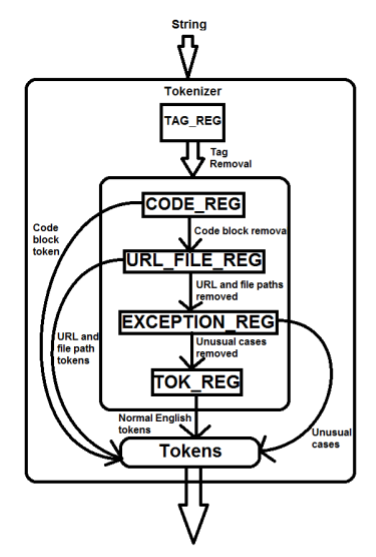
\includegraphics[width=0.9\linewidth]{tokenizer}
\caption{Tokenizer implementation}\label{img:tok}
\end{figure}

The implementation is given in \texttt{source\_code/tokenizer.py} under function
\texttt{tokenize\_v2\,()}.
TAG\_REG removes the html tags in the string, while CODE\_REG takes an entire code
block as a token. URL\_FILE\_REG then identifies the URLs and file paths (both Unix
and Windows) from the string. EXCEPTION\_REG identifies the tokens which are not
found in the English language (some examples are in Table~\ref{tok}). Finally,
TOK\_REG tokenizes the conventional English language words.

We have also written another function, \texttt{evaluate\,()} to evaluate
a tokenizer output against its ground truth, and output precision, recall and
F1 score.

To verify the correctness of our tokenizer, a testing script is written
(\texttt{source\_code/test.py}). This
script asserts the tokenizer for given test strings against expected tokenizer
outputs, allowing us to identify wrong cases to iteratively improve the tokenizer.
At the end of testing, the number of errors will be returned; the current
implementation is expected to pass all tests.

\section{Further Analysis and Annotation}

\section{Application}